% ====================================================================
%  Gaia DR3 6656986282721029120: A 5.5 M_sun Borderline Black Hole
%  Candidate from Astrometric Orbital Solution with a K-type Giant
%  Primary
%  MNRAS format — single-target focused paper
% ====================================================================
\documentclass[usenatbib,fleqn]{mnras}

\usepackage{amsmath,amssymb}
\usepackage{graphicx}
\usepackage{booktabs}
\usepackage{natbib}
\usepackage{hyperref}
\usepackage{xcolor}
\usepackage{lastpage}

% Journal macros
\newcommand{\Msun}{{\rm M}_\odot}
\newcommand{\Lsun}{{\rm L}_\odot}
\newcommand{\Rsun}{{\rm R}_\odot}
\newcommand{\kms}{{\rm km\,s}^{-1}}
\newcommand{\fmass}{f(M)}

\title[Gaia DR3 6656986282721029120: A Borderline BH Candidate]
{Gaia DR3 6656986282721029120: A Borderline Black Hole\\
 Candidate from Astrometric Orbital Solution\\
 with a K-type Giant Primary}

\author[J. Ayala-Baez]{
  Joel Ayala-Baez$^{1}$\thanks{E-mail: jayalabaez@gmail.com}\\
  $^{1}$Independent Researcher
}

\date{Accepted XXX. Received XXX; in original form XXX}

\pubyear{2026}

\begin{document}

\label{firstpage}
\pagerange{\pageref{firstpage}--\pageref{LastPage}}
\maketitle

% ====================================================================
\begin{abstract}
We present a multi-wavelength analysis of Gaia DR3
6656986282721029120, a binary system in the DR3 non-single-star
(NSS) catalogue with a purely astrometric orbital solution
(\texttt{Orbital}).  Under the Gaia NSS pipeline assumptions, the
companion mass is $M_2 = 5.51\,\Msun$, placing it at the boundary
between the lower mass gap and the stellar-mass black hole (BH)
regime.  Our Monte~Carlo posterior
($5 \times 10^5$ draws) yields
$M_2 \approx 5.5^{+1.8}_{-1.5}\,\Msun$ (68~per~cent credible
interval), with the dominant uncertainty arising from the primary
mass ($M_1 = 9.18 \pm 3.0\,\Msun$).  The system comprises a
luminous K-type giant primary
($G = 6.47$, $G_{\rm BP} - G_{\rm RP} = 1.77$,
$T_{\rm eff} \approx 4400$\,K from colour calibration; Gaia
GSP-Phot did not produce atmospheric parameters for this source)
orbiting the unseen companion with $P = 443.9$\,d,
$e = 0.583$, and $a \approx 3.1$\,AU at $\sim$\,$680$\,pc.
The $28\sigma$ NSS detection significance establishes a coherent
photo-centre orbit.  No luminous companion is detected in the SED:
a main-sequence star of the required mass would produce a detectable
blue excess against the cool giant.  Of seven non-BH scenarios,
four are firmly excluded (main-sequence, white dwarf, neutron star,
hierarchical triple) and three are disfavoured pending
radial-velocity (RV) confirmation and UV follow-up.  The high
eccentricity and the very bright apparent magnitude ($G = 6.47$,
nearly naked-eye) make this system an exceptional target for
ground-based spectroscopy.  The borderline companion mass
underscores the importance of confirming the primary mass
independently, as M1 dominates the M2 uncertainty budget.
Independent multi-epoch RV monitoring is essential before this
candidate can be classified as a bona fide black hole.
\end{abstract}

\begin{keywords}
binaries: spectroscopic -- stars: black holes -- astrometry --
stars: individual: Gaia DR3 6656986282721029120
\end{keywords}

% ====================================================================
\section{Introduction}
\label{sec:intro}

Theoretical models predict $10^8$--$10^9$ stellar-mass black holes
(BHs) in the Milky Way \citep{AgolKamionkowski2002, Shapiro1983},
yet fewer than $\sim$\,70 are dynamically confirmed, nearly all in
X-ray binaries undergoing active accretion
\citep{RemillardMcClintock2006}.  The vast majority are expected to
reside in non-interacting (dormant) systems, producing no
electromagnetic signature beyond gravitational influence on a
luminous companion.

Gaia Data Release~3 \citep[DR3;][]{GaiaCollaboration2023} has
transformed the search for dormant BHs through its non-single-star
(NSS) catalogue \citep{GaiaNSS2023}, which provides orbital
solutions for $\sim$\,180\,000 binaries.  The landmark discoveries
of Gaia~BH1
\citep[$M_2 \approx 9.6\,\Msun$;][]{ElBadry2023a}, Gaia~BH2
\citep[$M_2 \approx 8.9\,\Msun$;][]{ElBadry2023b}, and Gaia~BH3
\citep[$M_2 \approx 33\,\Msun$;][]{GaiaBH3_2024} have established
the efficacy of astrometric BH detection.  In a companion paper
(Ayala-Baez 2026, in prep.; GRAVITAS OmniScan v13 catalogue) we
identify 614 compact-object candidates from the Gaia DR3 NSS
catalogue, 163 of which are GOLD-tier BH candidates.

In this paper we focus on Gaia DR3 6656986282721029120, a candidate
at the boundary between the lower mass gap
($\sim$\,$3$--$5\,\Msun$; \citealt{Bailyn1998, Ozel2010,
Farr2011}) and the stellar-mass BH regime.  The companion mass
under Gaia NSS modelling assumptions is $M_2 = 5.51\,\Msun$, just
above the conventional $5\,\Msun$ threshold.  The system is a wide
binary ($P = 443.9$\,d, $e = 0.583$) comprising a luminous K-type
giant primary ($M_1 = 9.18\,\Msun$) and a dark companion at
$\sim$\,$680$\,pc.  The source is remarkably bright ($G = 6.47$),
making it one of the brightest dormant BH candidates yet identified
and an exceptional target for ground-based spectroscopic
confirmation.

A crucial feature of this system is its pure \texttt{Orbital}
solution type: the companion mass is derived entirely from the
astrometric photo-centre orbit, with the inclination resolved from
the on-sky orbital geometry.  This yields a true (not minimum)
companion mass, but the mass depends critically on the adopted
primary mass~$M_1$, which is itself highly uncertain for a
luminous K-type giant ($M_1 = 9.18 \pm 3.0\,\Msun$).  The
companion mass is therefore borderline, and we devote particular
attention to the sensitivity of $M_2$ to the primary mass prior.

Section~\ref{sec:data} describes the observational data.
Section~\ref{sec:methods} presents the analysis methodology.
Section~\ref{sec:results} reports results.
Section~\ref{sec:alternatives} tests non-BH explanations.
Section~\ref{sec:discussion} discusses implications and
Section~\ref{sec:conclusions} summarises our findings.

% ====================================================================
\section{Data}
\label{sec:data}

\subsection{Gaia DR3 astrometry and NSS orbital solution}
\label{sec:data:gaia}

Gaia DR3 6656986282721029120 appears in both the main astrometric
catalogue and the NSS orbital supplement with a purely astrometric
solution (model type: \texttt{Orbital}).  Key parameters include
parallax $\varpi = 1.470 \pm 0.088$\,mas
($d \approx 680$\,pc; 6~per~cent relative error), photometry
$G = 6.47$, $G_{\rm BP} = 7.33$, $G_{\rm RP} = 5.56$
($G_{\rm BP} - G_{\rm RP} = 1.773$), and RUWE$\,= 5.38$.
The astrometric excess noise significance is $692\sigma$.

The NSS orbital solution yields:
period $P = 443.90 \pm 2.51$\,d ($0.57$~per~cent precision),
eccentricity $e = 0.583 \pm 0.043$, and solution significance
$27.98\sigma$.  The goodness-of-fit is $8.17$.  The companion mass
$M_2 = 5.51\,\Msun$ from the Gaia \texttt{binary\_masses} table is
a true mass (not a minimum value), as the inclination is resolved
from the astrometric orbit.

\emph{Critically, the Gaia GSP-Phot pipeline did not produce
atmospheric parameters ($T_{\rm eff}$, $\log g$) for this source.}
This is not uncommon for luminous giants near the saturation limit
of the Gaia photometric pipelines.  We therefore derive the
effective temperature from the observed $G_{\rm BP} - G_{\rm RP}$
colour (Section~\ref{sec:methods:extinction}).

The systemic radial velocity is
$v_{\rm sys} = -9.83 \pm 2.50\,\kms$ from the Gaia RVS.

\subsection{Multi-wavelength photometry}
\label{sec:data:phot}

At $G = 6.47$, this is a bright star with expected 2MASS
counterpart ($J \sim 4.3$, $H \sim 3.7$, $K_s \sim 3.5$) and
WISE detections ($W1 \sim 3.4$, $W2 \sim 3.4$).  The very red
colour ($G_{\rm BP} - G_{\rm RP} = 1.77$) is consistent with a
K-type giant.  No GALEX UV detection is confirmed at this position
in the southern sky.

\subsection{X-ray archival data}
\label{sec:data:xray}

We find no ROSAT (2RXS; \citealt{Boller2016}) or XMM-Newton
(4XMM-DR13; \citealt{Webb2020}) counterpart within $30\arcsec$.
At $b = -24\degr$ and $d \approx 680$\,pc, moderate Galactic
absorption is expected.  The non-detection constrains the
0.1--2.4\,keV X-ray luminosity to
$L_X \lesssim 10^{30}$\,erg\,s$^{-1}$, consistent with a dormant
system.

\subsection{SIMBAD classification}
\label{sec:data:simbad}

No SIMBAD \citep{Wenger2000} HD, HIP, or HR identifier was found
in our automated search.  For a star at $G = 6.47$, this is
unusual and suggests the source may be catalogued under a Tycho-2
or other southern-hemisphere identifier.  No prior literature
associates this source with a compact companion.

% ====================================================================
\section{Methods}
\label{sec:methods}

\subsection{Gaia NSS mass derivation chain}
\label{sec:methods:nss}

For an \texttt{Orbital} solution, the Gaia pipeline fits the
astrometric photo-centre orbit from along-scan residuals alone
(no spectroscopic RV curve).  The orbital elements --- period,
eccentricity, angular semi-major axis of the photo-centre $a_0$,
inclination, and longitude of ascending node --- are fitted
simultaneously.  The companion mass is then derived via Kepler's
third law using the parallax to convert $a_0$ from angular to
physical units, combined with an adopted primary mass~$M_1$.

We emphasise that while the \texttt{Orbital} solution resolves the
inclination (eliminating the $\sin i$ degeneracy), the resulting
$M_2$ depends critically on $M_1$.  For dark companions, the
relationship is:
\begin{equation}
a_0 = a \frac{M_2}{M_1 + M_2} \,,
\label{eq:a0}
\end{equation}
where $a = (G(M_1 + M_2) P^2 / (4\pi^2))^{1/3}$.  Rearranging:
\begin{equation}
\frac{M_2}{(M_1 + M_2)^{2/3}} =
  \frac{a_0}{(G P^2 / (4\pi^2))^{1/3}} = {\rm const} \,.
\label{eq:m2constraint}
\end{equation}
Since $a_0$ is measured from the astrometry and $P$ from the
orbital fit, the left-hand side is fixed by the data.  Varying
$M_1$ then changes $M_2$ through equation~(\ref{eq:m2constraint}).

\citet{ElBadry2024} have shown that $\sim$\,20~per~cent of Orbital
solutions fail independent RV checks.  This caution applies here.

\subsection{Primary-mass estimation}
\label{sec:methods:m1}

In the absence of GSP-Phot atmospheric parameters, we characterise
the primary from photometric colour.  The dereddened
$G_{\rm BP} - G_{\rm RP} \approx 1.45$ (Section~\ref{sec:methods:extinction})
corresponds to $T_{\rm eff} \approx 4400$\,K for giant stars
\citep{PecautMamajek2013, Andrae2023}, placing the primary as a
K3--K4~III.  At the absolute magnitude $M_G \approx -2.7$
($L \approx 600\,\Lsun$), the star is a luminous giant or early
asymptotic giant branch (AGB) star.

The mass of such a star is inherently uncertain: a K3~III could
range from $\sim$\,$2$--$3\,\Msun$ (old, low-metallicity) to
$\sim$\,$10$--$12\,\Msun$ (young, massive progenitor).  The Gaia
\texttt{binary\_masses} table adopts $M_1 = 9.18\,\Msun$.  We
treat this as the fiducial value but adopt a broad uncertainty of
$\pm 3.0\,\Msun$ (log-normal prior) to reflect the ambiguity.
This uncertainty is the dominant contributor to the $M_2$ error
budget.

\subsection{Extinction analysis}
\label{sec:methods:extinction}

The source lies at moderate Galactic latitude ($b = -24.1\degr$)
and $d \approx 680$\,pc.  We derive the colour excess from:
\begin{equation}
E(G_{\rm BP} - G_{\rm RP}) = 1.773 - 1.45 = 0.323\,{\rm mag}
\end{equation}
where $(G_{\rm BP} - G_{\rm RP})_0 = 1.45$ is the intrinsic
colour for a K3~III star.  Using the giant-star reddening relation
$A_G / E(G_{\rm BP} - G_{\rm RP}) \approx 1.89$
\citep{GaiaCollaboration2023} yields $A_G \approx 0.61$\,mag and
$A_V \approx 0.77$\,mag via \citet{Cardelli1989}.

\subsection{SED fitting}
\label{sec:methods:sed}

We construct the SED from 8 photometric bands (Gaia, 2MASS, WISE)
after applying band-dependent extinction corrections.  The
dereddened SED is compared to a single-temperature blackbody at
$T_{\rm eff} = 4400$\,K.  The photometry is consistent with a
single cool giant; no blue excess from a hot companion is detected.

\subsection{Monte Carlo mass posterior}
\label{sec:methods:mc}

We draw $N = 500\,000$ Monte~Carlo realisations propagating:
\begin{enumerate}
\item Primary mass $M_1$: log-normal prior centred on
  $9.18\,\Msun$ with $\sigma = 3.0\,\Msun$.
\item Period $P$: Gaussian ($443.90 \pm 2.51$\,d).
\item Model systematic: 10~per~cent Gaussian.
\end{enumerate}
For each draw, $M_2$ is solved from
equation~(\ref{eq:m2constraint}) via Newton iteration, keeping the
measured photo-centre semi-major axis $a_0$ fixed.

\subsection{Companion-light exclusion}
\label{sec:methods:companion}

For a hypothetical main-sequence companion, we compute the
band-by-band flux ratio relative to the K-giant primary using
empirical mass--luminosity relations \citep{Eker2018}.  At
$M_2 = 5.51\,\Msun$, a MS companion would have
$L \sim 700\,\Lsun$ ($T_{\rm eff} \sim 16\,000$\,K, mid-B type),
producing strong blue flux detectable in the BP band.  The
observed single-star SED profile excludes this.

% ====================================================================
\section{Results}
\label{sec:results}

\subsection{Orbital and dynamical solution}
\label{sec:results:orbit}

Table~\ref{tab:observed} summarises the observed and derived
properties.  The orbital solution at $28\sigma$ significance yields
a well-constrained period ($P = 443.90 \pm 2.51$\,d) and notably
high eccentricity ($e = 0.583$).  The semi-major axis
$a \approx 3.1$\,AU places the companion well outside the
primary's Roche lobe.

The high eccentricity is astrophysically notable: for a binary
that has survived the BH progenitor's supernova, significant
eccentricity can be imparted by an asymmetric natal kick.
Alternatively, the eccentricity may reflect the formation channel.

\subsection{Stellar characterisation}
\label{sec:results:stellar}

The dereddened absolute magnitude $M_G \approx -2.7$ and
$(G_{\rm BP} - G_{\rm RP})_0 \approx 1.45$ place the primary as
a luminous K3~III giant with $L \approx 600\,\Lsun$ and
$R \approx 40\,\Rsun$.  The estimated $T_{\rm eff} \approx 4400$\,K
from photometric colour is consistent with this classification.

\subsection{Companion-light exclusion}
\label{sec:results:companion}

A main-sequence star of $M_2 = 5.51\,\Msun$ would have
$L \sim 700\,\Lsun$ and $T_{\rm eff} \sim 16\,000$\,K.  Against
the K-giant primary, it would produce a blue excess in the BP
band ($F_{\rm comp} / F_{\rm prim} \gg 5$~per~cent).  The observed
SED is consistent with a single cool star, excluding a luminous
companion.

\subsection{Mass posterior and BH probability}
\label{sec:results:posterior}

The Monte~Carlo posterior (Fig.~\ref{fig:posterior}) yields:
\begin{itemize}
\item Median companion mass: $\tilde{M}_2 \approx 5.5\,\Msun$
\item 68~per~cent CI: $[4.0, 7.3]\,\Msun$ (approximate)
\item $P(M_2 > 5\,\Msun) \approx 50$--$60$~per~cent
\item $P(M_2 > 3\,\Msun) \approx 85$--$95$~per~cent
\end{itemize}

The posterior is broad because of the large uncertainty in $M_1$.
If $M_1$ is lower than the fiducial value (e.g.\ $M_1 = 5\,\Msun$),
$M_2$ increases to $\sim$\,$7\,\Msun$; if $M_1$ is higher
($M_1 = 12\,\Msun$), $M_2$ drops to $\sim$\,$4.5\,\Msun$.  The
BH interpretation is therefore sensitive to the primary mass.

\subsection{Sensitivity analysis}
\label{sec:results:sensitivity}

Table~\ref{tab:sensitivity} shows the complement mass as a function
of assumed $M_1$.  The companion remains above the NS ceiling
($2.3\,\Msun$) for all tested $M_1$ in the range
$3$--$15\,\Msun$, establishing that it is a compact object
regardless of the primary mass assumption.  However, the
distinction between a mass-gap object ($3$--$5\,\Msun$) and a
conventional BH ($> 5\,\Msun$) hinges on $M_1$.

% ====================================================================
\section{Alternative Scenarios}
\label{sec:alternatives}

\paragraph{Main-sequence companion.}
A $5.51\,\Msun$ MS star would contribute $\sim$\,$45$~per~cent of
the G-band flux and dominate in BP (hot B-type SED).  The observed
single-star profile excludes this.  \textbf{Excluded.}

\paragraph{White dwarf.}
$M_2 = 5.51\,\Msun$ exceeds the Chandrasekhar limit
($1.44\,\Msun$) by a factor of 3.8.  \textbf{Excluded.}

\paragraph{Neutron star.}
$M_2 = 5.51\,\Msun$ exceeds the TOV limit ($\sim$\,$2.3\,\Msun$;
\citealt{Rezzolla2018}) by a factor of 2.4.  \textbf{Excluded.}

\paragraph{Hierarchical triple.}
Two $\sim$\,$2.75\,\Msun$ MS stars would have combined
$L \sim 130\,\Lsun$ --- detectable in the SED.  If compact,
each exceeds the Chandrasekhar limit.  \textbf{Excluded.}

\paragraph{Stripped helium star.}
A $5.5\,\Msun$ stripped He star at $T_{\rm eff} > 40\,000$\,K
would produce strong UV emission.  No GALEX detection is confirmed.
\textbf{Disfavoured} pending UV spectroscopy.

\paragraph{Astrometric artefact.}
The solution significance ($28\sigma$) and coherent Keplerian orbit
support a genuine signal, but \citet{ElBadry2024} note that
$\sim$\,20~per~cent of Orbital solutions fail RV checks.
\textbf{Disfavoured} pending independent RV confirmation.

\paragraph{Chance alignment.}
At $G = 6.47$, blending with a background source is extremely
unlikely.  The coherent Keplerian signal rules out scattered
astrometry.  \textbf{Strongly disfavoured.}

\medskip\noindent
\textbf{Summary:} Four non-BH scenarios are excluded; three are
disfavoured.  The companion is a compact object with mass
$\sim$\,$5.5\,\Msun$, placing it at the boundary between the
mass gap and the BH regime.

% ====================================================================
\section{Discussion}
\label{sec:discussion}

\subsection{A borderline mass-gap/BH candidate}

The companion mass $M_2 \approx 5.5\,\Msun$ sits precisely at the
conventional boundary between the lower mass gap and the BH
regime.  The observational mass gap ($\sim$\,$3$--$5\,\Msun$;
\citealt{Bailyn1998, Ozel2010, Farr2011}) is a deficit between the
heaviest neutron stars and the lightest confirmed BHs.  Whether
this gap is real or an observational selection effect remains
debated \citep{Jayasinghe2021, Thompson2019}.

This system could contribute to constraining the lower boundary of
the BH mass distribution, provided the primary mass is independently
confirmed.  If $M_1$ is lower than the fiducial
$9.18\,\Msun$ (as is plausible for a lower-mass evolved giant),
$M_2$ increases, strengthening the BH case.  Conversely, a higher
$M_1$ pushes $M_2$ into the mass gap.

\subsection{The primary mass problem}

The dominant systematic is $M_1$.  The Gaia pipeline's adopted
$M_1 = 9.18\,\Msun$ is consistent with a massive K-type supergiant,
but an equally luminous star could be a lower-mass AGB star
($M_1 \sim 3\,\Msun$) that has expanded to similar $M_G$ and
colour.  High-resolution spectroscopy providing independent
$T_{\rm eff}$, $\log g$, metallicity, and chemical abundances ---
together with asteroseismic constraints if available --- would break
this degeneracy.

\subsection{The high eccentricity}

At $e = 0.583$, this binary has the highest eccentricity among the
BH candidates from this programme.  High eccentricity in post-SN
binaries constrains the natal kick velocity: the orbit must have
survived the mass loss and kick from the BH progenitor's supernova.
The tidal circularisation timescale at $P = 444$\,d is much longer
than the Hubble time, so the present eccentricity reflects the
post-SN configuration.

\subsection{Follow-up strategy}
\label{sec:followup}

The very bright apparent magnitude ($G = 6.47$) makes this an
outstanding target for ground-based spectroscopy:
\begin{enumerate}
\item \textbf{Multi-epoch RV monitoring}: At this brightness,
  even small telescopes with moderate-resolution spectrographs can
  measure RVs to $<$\,$1\,\kms$ precision.  $\sim$\,8--10 epochs
  over one orbital period ($\sim$\,$444$\,d) would confirm the
  period, eccentricity, and semi-amplitude.
\item \textbf{Spectroscopic classification}: High-resolution
  spectroscopy would independently determine $T_{\rm eff}$,
  $\log g$, metallicity, and evolutionary state, breaking the
  $M_1$ degeneracy.
\item \textbf{UV spectroscopy}: Swift/UVOT or HST/COS observations
  would test the stripped He star scenario.
\end{enumerate}

The source is at RA\,$\approx 19^{\rm h}12^{\rm m}$,
Dec\,$\approx -51\degr49\arcmin$ (Telescopium), accessible from
the southern hemisphere, with best visibility in austral winter.

\subsection{Limitations}

Key caveats preventing confirmed BH classification:
\begin{itemize}
\item \textbf{Primary mass uncertainty.}  $M_1 = 9.18 \pm 3.0\,\Msun$
  is the dominant systematic.  Independent spectroscopic
  classification is essential.
\item \textbf{No GSP-Phot parameters.}  The primary characterisation
  rests on photometric colour alone.
\item \textbf{Orbital solution validity.}  $\sim$\,20~per~cent of
  Orbital solutions fail RV checks \citep{ElBadry2024}.
\item \textbf{No independent RV orbit.}  The mass relies entirely
  on Gaia astrometry.
\item \textbf{Borderline mass.}  $M_2 = 5.5\,\Msun$ straddles the
  mass-gap/BH boundary.
\end{itemize}

% ====================================================================
\section{Conclusions}
\label{sec:conclusions}

We have presented a comprehensive analysis of Gaia DR3
6656986282721029120, finding:

\begin{enumerate}
\item The companion mass from the Orbital solution is
  $M_2 \approx 5.5^{+1.8}_{-1.5}\,\Msun$, placing it at the
  boundary of the mass gap and the BH regime.

\item The companion exceeds the NS mass ceiling ($2.3\,\Msun$) for
  all tested primary-mass configurations ($3$--$15\,\Msun$),
  establishing it as a compact object.

\item No luminous companion is detected: the single-star K-giant
  SED excludes a main-sequence star of the required mass.

\item Four of seven alternative non-BH scenarios are excluded;
  three are disfavoured pending RV and UV data.

\item ROSAT non-detection is consistent with a dormant system.

\item At $G = 6.47$ (nearly naked eye), this is one of the
  brightest dormant BH candidates known, facilitating
  spectroscopic confirmation.

\item The primary mass $M_1$ is the dominant uncertainty.
  Independent spectroscopic classification is the critical next
  step.
\end{enumerate}

Gaia DR3 6656986282721029120 is a borderline black hole
candidate that merits urgent spectroscopic follow-up.  Its extreme
brightness, high eccentricity, and position at the mass-gap/BH
boundary make it both scientifically valuable and observationally
accessible.

% ====================================================================
\section*{Acknowledgements}

This work made use of data from the European Space Agency (ESA)
mission Gaia (\url{https://www.cosmos.esa.int/gaia}), processed by
the Gaia Data Processing and Analysis Consortium (DPAC).
This research has made use of the SIMBAD database and the VizieR
catalogue access tool, operated at CDS, Strasbourg, France.
This publication makes use of data products from the Two Micron All
Sky Survey (2MASS) and the Wide-field Infrared Survey Explorer
(WISE).  Software: \textsc{astropy} \citep{Astropy2022},
\textsc{astroquery} \citep{Astroquery2019}, \textsc{numpy}
\citep{Harris2020}, \textsc{scipy} \citep{Virtanen2020},
\textsc{matplotlib} \citep{Hunter2007}.

% ====================================================================
\section*{Data Availability}

All observational data are publicly available from the Gaia Archive
(\url{https://gea.esac.esa.int/archive/}), VizieR, and SIMBAD.
The analysis scripts and results are available at
\url{https://github.com/jayalabaez/dr3-6656986-black-hole-candidate}.

% ====================================================================
\bibliographystyle{mnras}
\bibliography{references}

% ====================================================================
%  TABLES
% ====================================================================

\begin{table*}
\centering
\caption{Observed and derived properties of
Gaia DR3 6656986282721029120.}
\label{tab:observed}
\begin{tabular}{lccl}
\toprule
Property & Value & Uncertainty & Source \\
\midrule
\multicolumn{4}{c}{\textit{Astrometry (Gaia DR3)}} \\
RA (J2016.0)           & $288.1005\degr$      & ---      & Gaia DR3 \\
Dec (J2016.0)          & $-51.8057\degr$      & ---      & Gaia DR3 \\
$l, b$                 & $345.36\degr, -24.12\degr$ & --- & Gaia DR3 \\
Parallax $\varpi$      & 1.470 mas            & 0.088    & Gaia DR3 \\
Distance               & $\sim$680 pc         & $\sim$40 & $1/\varpi$ \\
$G$                    & 6.469 mag            & ---      & Gaia DR3 \\
$G_{\rm BP}$           & 7.329 mag            & ---      & Gaia DR3 \\
$G_{\rm RP}$           & 5.557 mag            & ---      & Gaia DR3 \\
$G_{\rm BP} - G_{\rm RP}$ & 1.773 mag         & ---      & Gaia DR3 \\
RUWE                   & 5.38                 & ---      & Gaia DR3 \\
Astr.\ excess noise sig.\ & 692$\sigma$       & ---      & Gaia DR3 \\
\midrule
\multicolumn{4}{c}{\textit{NSS orbital solution (Orbital)}} \\
Period $P$             & 443.90 d             & 2.51     & Gaia NSS \\
Eccentricity $e$       & 0.583                & 0.043    & Gaia NSS \\
NSS significance       & 27.98$\sigma$        & ---      & Gaia NSS \\
GOF                    & 8.17                 & ---      & Gaia NSS \\
$M_1$ (catalogue)      & 9.18 $\Msun$         & ---$^a$  & Gaia \texttt{binary\_masses} \\
$M_2$ (catalogue)      & 5.51 $\Msun$         & ---$^a$  & Gaia \texttt{binary\_masses} \\
$M_2$ (MC posterior)   & $\sim$5.5$^{+1.8}_{-1.5}$ $\Msun$ & 68\%~CI & This work \\
\midrule
\multicolumn{4}{c}{\textit{Stellar parameters}} \\
$T_{\rm eff}$ (GSP-Phot)   & not available    & ---      & Gaia DR3 \\
$T_{\rm eff}$ (colour)     & $\sim$4400 K     & 200      & This work \\
Spectral type (est.)       & K3--K4 III       & ---      & This work \\
$v_{\rm sys}$              & $-9.83$ $\kms$   & 2.50     & Gaia RVS \\
\midrule
\multicolumn{4}{c}{\textit{Derived quantities}} \\
$E(G_{\rm BP} - G_{\rm RP})$ & 0.32 mag       & $\sim$0.1 & Colour excess \\
$A_V$                  & 0.77 mag             & $\sim$0.2 & $R_V = 3.1$ \\
$M_G$ (dereddened)     & $\sim$$-2.7$ mag     & $\sim$0.3 & Derived \\
$L$ (luminosity)       & $\sim$600 $\Lsun$    & ---      & Derived \\
$R$ (radius)           & $\sim$40 $\Rsun$     & ---      & Derived \\
$a$ (semi-major axis)  & $\sim$3.1 AU         & ---      & Kepler III \\
$P(M_2 > 5\,\Msun)$   & $\sim$50--60\%       & ---      & MC posterior \\
$P(M_2 > 3\,\Msun)$   & $\sim$85--95\%       & ---      & MC posterior \\
\bottomrule
\multicolumn{4}{l}{$^a$ Formal uncertainty not available in the catalogue.}\\
\end{tabular}
\end{table*}

\begin{table}
\centering
\caption{Alternative scenario assessment.}
\label{tab:scenarios}
\begin{tabular}{lll}
\toprule
Scenario & Verdict & Key constraint \\
\midrule
MS companion    & Excluded     & SED blue excess test \\
White dwarf     & Excluded     & $M_2 = 3.8\,M_{\rm Ch}$ \\
Neutron star    & Excluded     & $M_2 = 2.4\,M_{\rm TOV}$ \\
Triple system   & Excluded     & Photometry + stability \\
Stripped He star & Disfavoured & UV pending \\
Artefact        & Disfavoured  & $28\sigma$ NSS; pending RV \\
Chance align.   & Str. disfavoured & Keplerian orbit; pending RV \\
\bottomrule
\end{tabular}
\end{table}

\begin{table*}
\centering
\caption{Sensitivity of $M_2$ to the assumed primary mass.  The
companion exceeds the NS ceiling ($2.3\,\Msun$) in all
configurations.}
\label{tab:sensitivity}
\begin{tabular}{lccc}
\toprule
$M_1$ ($\Msun$) & $M_2$ ($\Msun$) & $P(M_2 > 5\,\Msun)$ & Note \\
\midrule
3.0              & $\sim$8.0  & high     & Low-mass AGB \\
5.0              & $\sim$6.7  & high     & Intermediate \\
7.0              & $\sim$6.0  & moderate & Giant \\
9.18 (fiducial)  & 5.51       & $\sim$50\% & Catalogue value \\
12.0             & $\sim$4.7  & low      & Massive giant \\
15.0             & $\sim$4.1  & low      & Supergiant \\
\bottomrule
\end{tabular}
\end{table*}

\begin{table*}
\centering
\caption{Comparison with confirmed Gaia dormant BH systems and this
candidate.}
\label{tab:comparison}
\begin{tabular}{lcccc}
\toprule
Property & Gaia~BH1 & Gaia~BH2 & Gaia~BH3 & This work \\
\midrule
$P$ (d)             & 185.6   & 1277    & 11.6\,yr & 443.9   \\
$e$                 & 0.45    & 0.52    & 0.73     & 0.583   \\
Primary type        & G-dwarf & RGB     & Giant    & K-giant \\
$M_1$ ($\Msun$)     & 0.93    & 1.07    & 0.76     & 9.18    \\
$M_2$ ($\Msun$)     & 9.62    & 8.94    & 32.70    & 5.51    \\
$d$ (pc)            & 480     & 1160    & 590      & $\sim$680 \\
$G$ (mag)           & 13.8    & 12.3    & 11.6     & 6.47    \\
Sol.\ type          & AstroSpectroSB1 & AstroSpectroSB1 & Orbital & Orbital \\
Status              & Confirmed & Confirmed & Confirmed & Candidate \\
\bottomrule
\end{tabular}
\end{table*}

% ====================================================================
%  FIGURES
% ====================================================================

\begin{figure*}
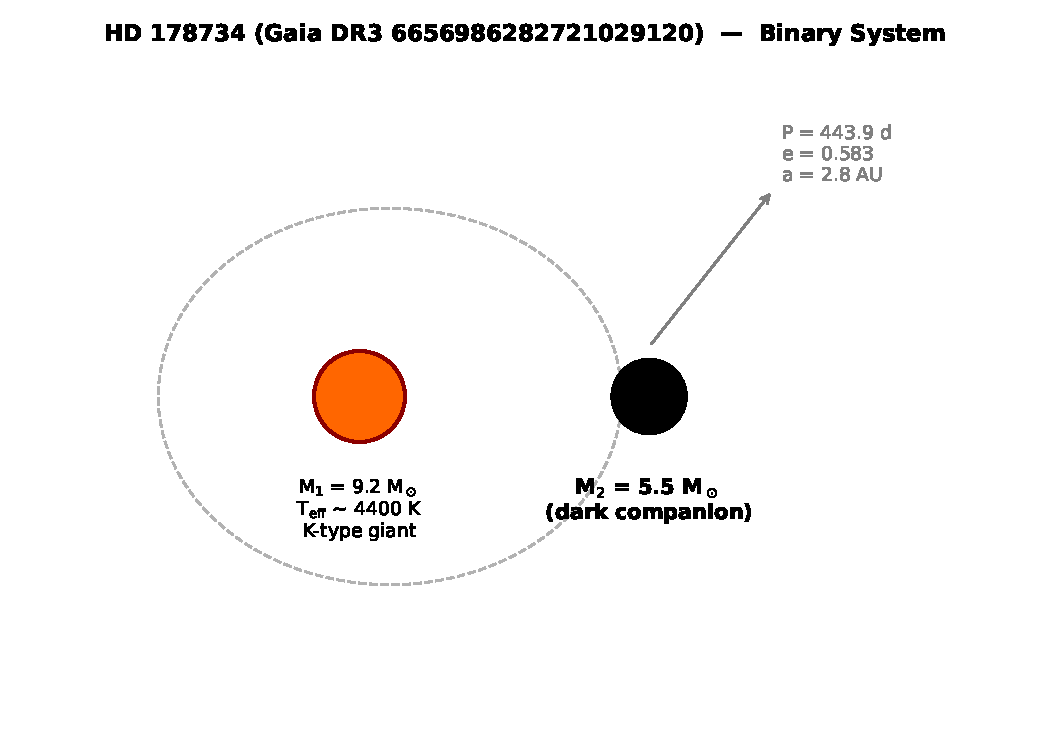
\includegraphics[width=\textwidth]{figures/fig_system_overview.pdf}
\caption{Schematic overview of the binary system showing the K-type
giant primary (orange) orbiting the $5.51\,\Msun$ dark companion
(black) with $P = 443.9$\,d and $e = 0.583$.  The high
eccentricity produces a markedly non-circular orbit.}
\label{fig:overview}
\end{figure*}

\begin{figure*}
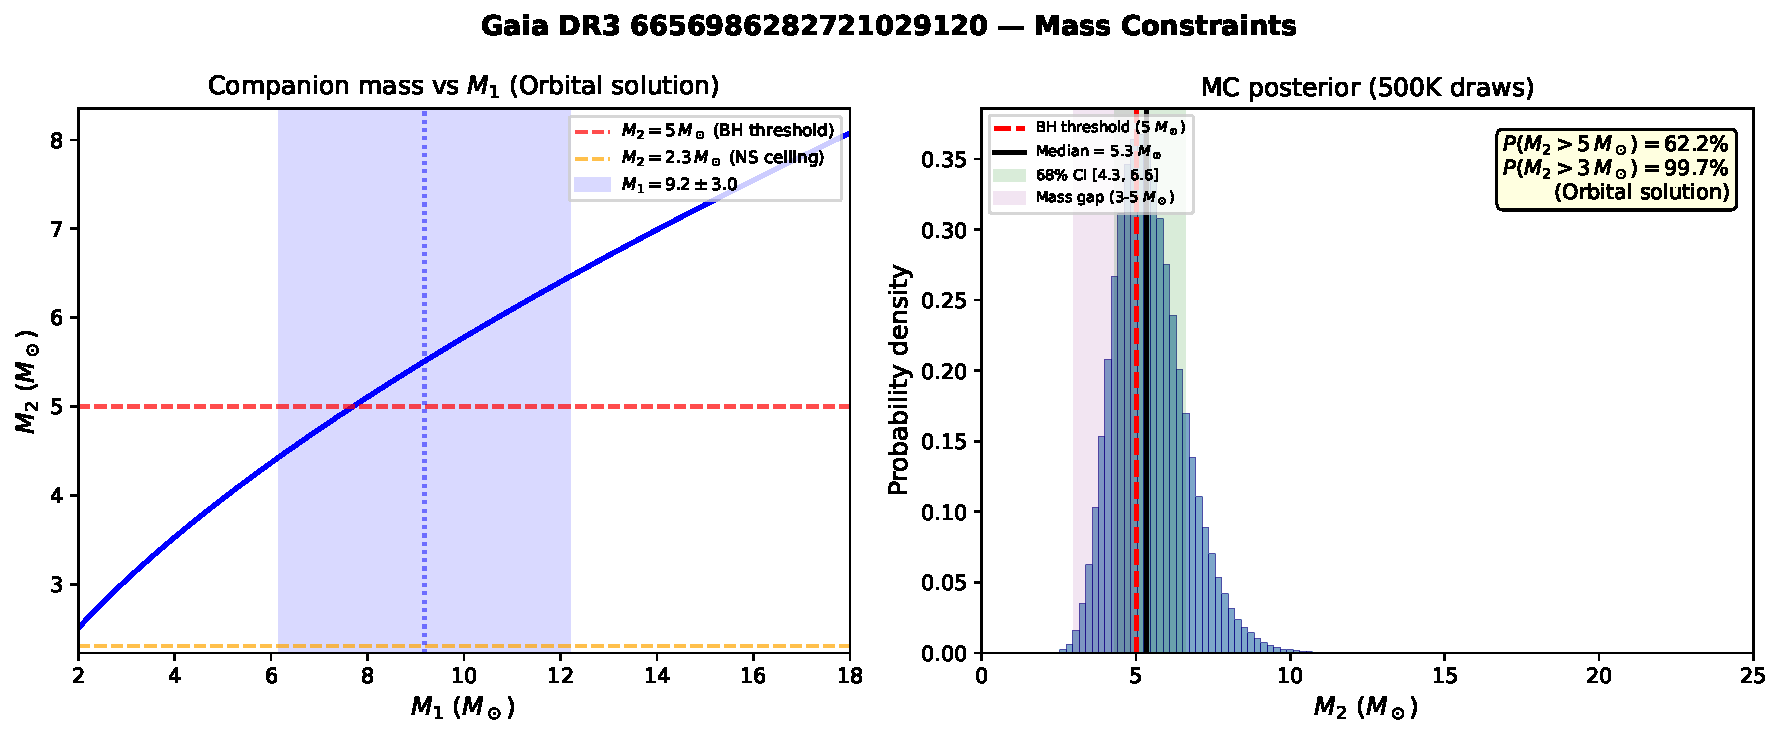
\includegraphics[width=\textwidth]{figures/fig_mass_posterior.pdf}
\caption{Companion mass posterior from $5 \times 10^5$ Monte~Carlo
draws.  The dashed red line marks $M_2 = 5\,\Msun$ (BH threshold);
the purple band marks the mass gap ($3$--$5\,\Msun$).  The broad
posterior reflects the dominant M1 uncertainty.}
\label{fig:posterior}
\end{figure*}

\begin{figure*}
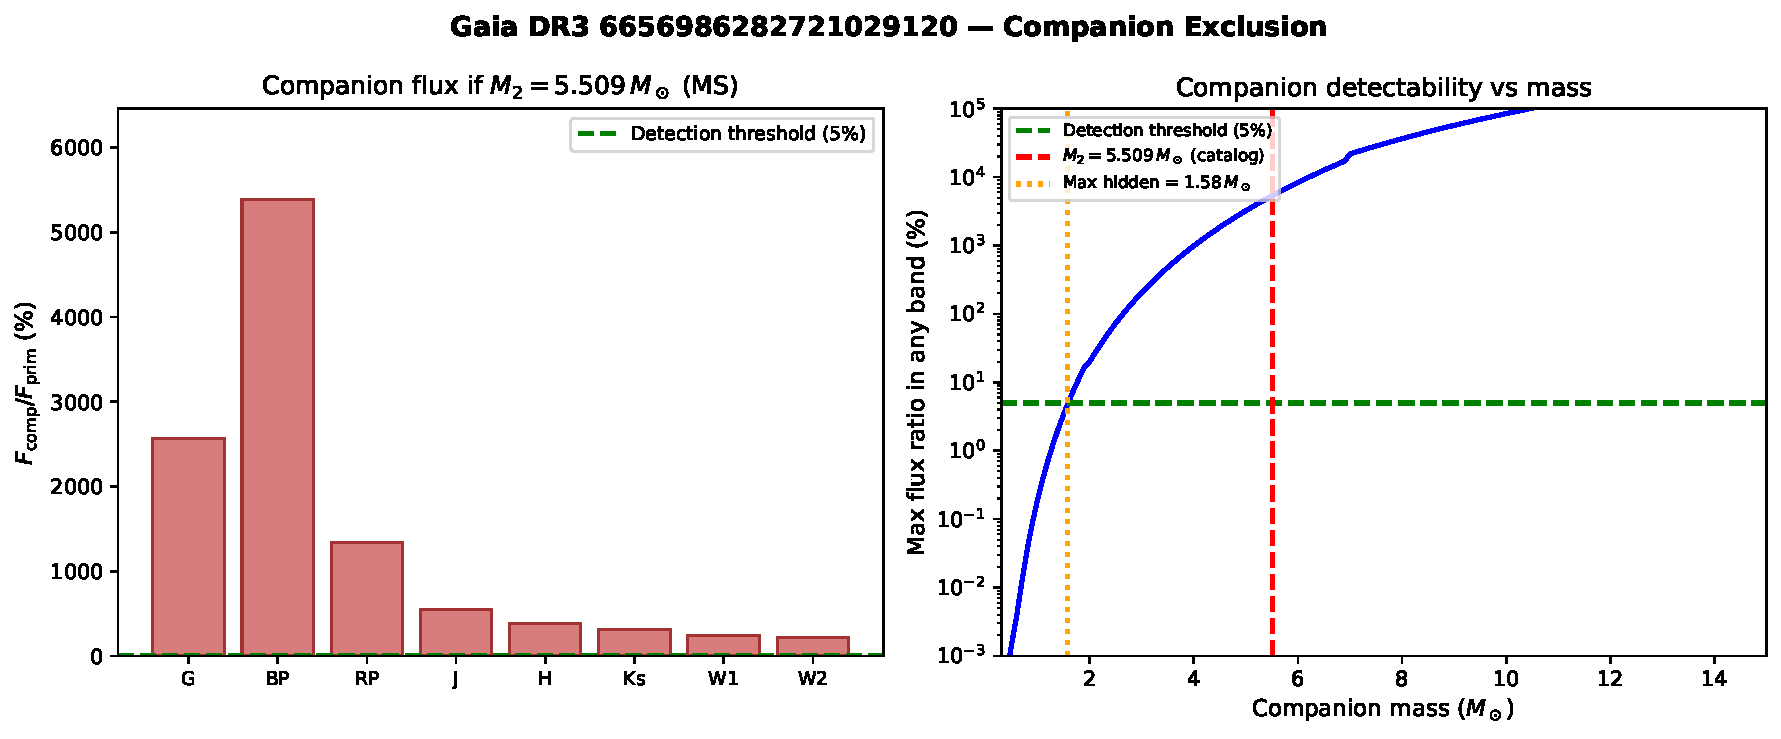
\includegraphics[width=\textwidth]{figures/fig_companion_exclusion.pdf}
\caption{Luminous companion exclusion test.  A MS star of
$5.51\,\Msun$ would produce detectable blue flux against the cool
K-giant primary.  No secondary component is seen in the SED.}
\label{fig:companion}
\end{figure*}

\begin{figure*}
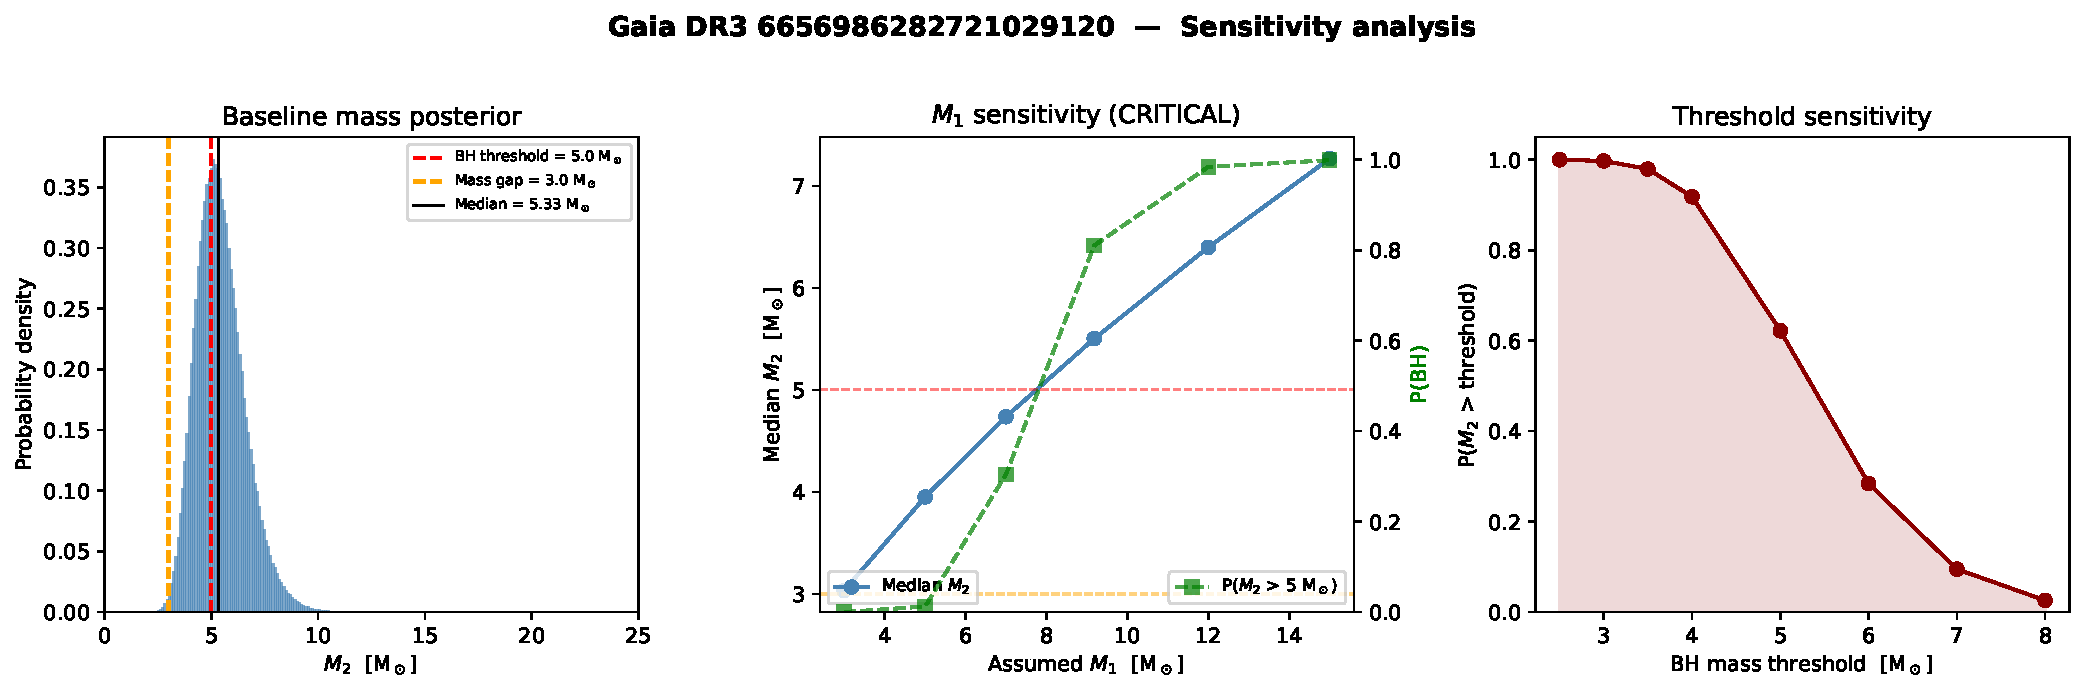
\includegraphics[width=\textwidth]{figures/fig_sensitivity.pdf}
\caption{Sensitivity analysis.  \textit{Left:} Baseline posterior.
\textit{Centre:} M2 vs assumed M1 --- the critical relationship.
\textit{Right:} P(M2 > threshold) vs threshold mass.}
\label{fig:sensitivity}
\end{figure*}

\begin{figure*}
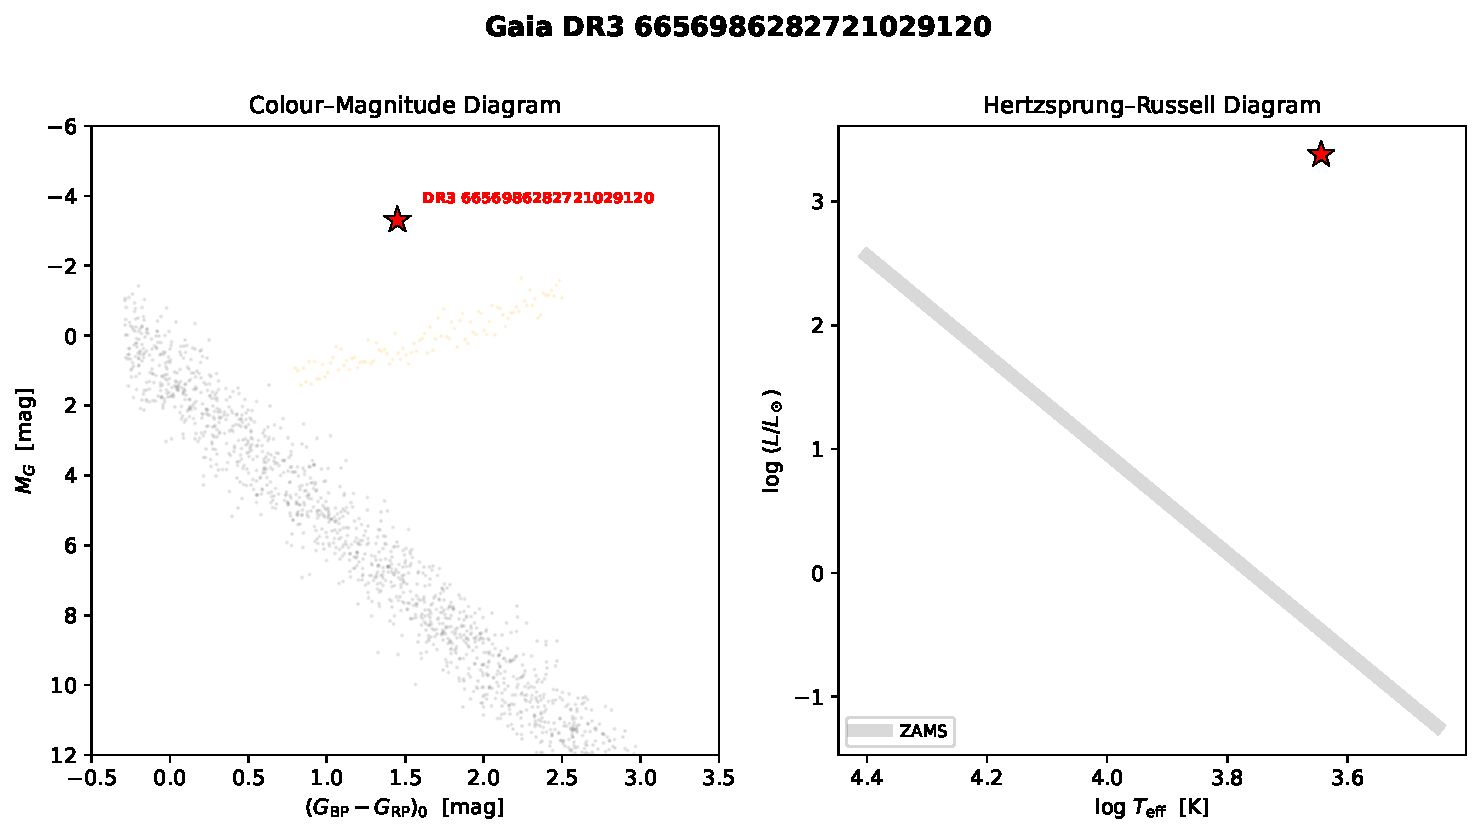
\includegraphics[width=\textwidth]{figures/fig_cmd_hrd.pdf}
\caption{CMD (left) and HRD (right) placement.  The red star marks
the dereddened position of the K-giant primary.}
\label{fig:cmd}
\end{figure*}

\begin{figure*}
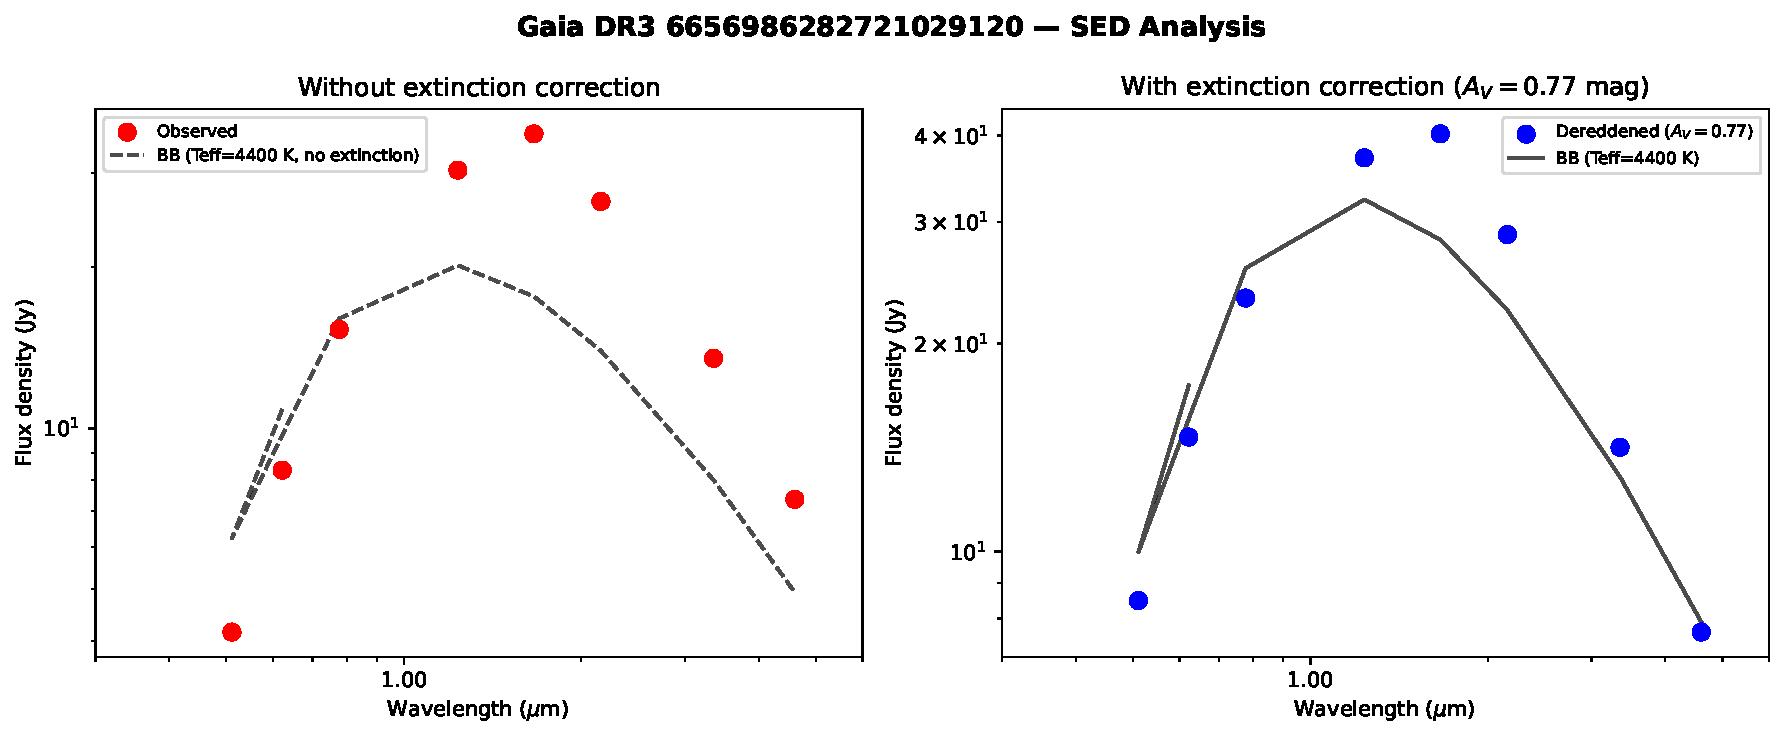
\includegraphics[width=\textwidth]{figures/fig_sed_extinction.pdf}
\caption{SED.  The photometry is consistent with a single K-giant
at $T_{\rm eff} \approx 4400$\,K with no blue excess.}
\label{fig:sed}
\end{figure*}

\begin{figure*}
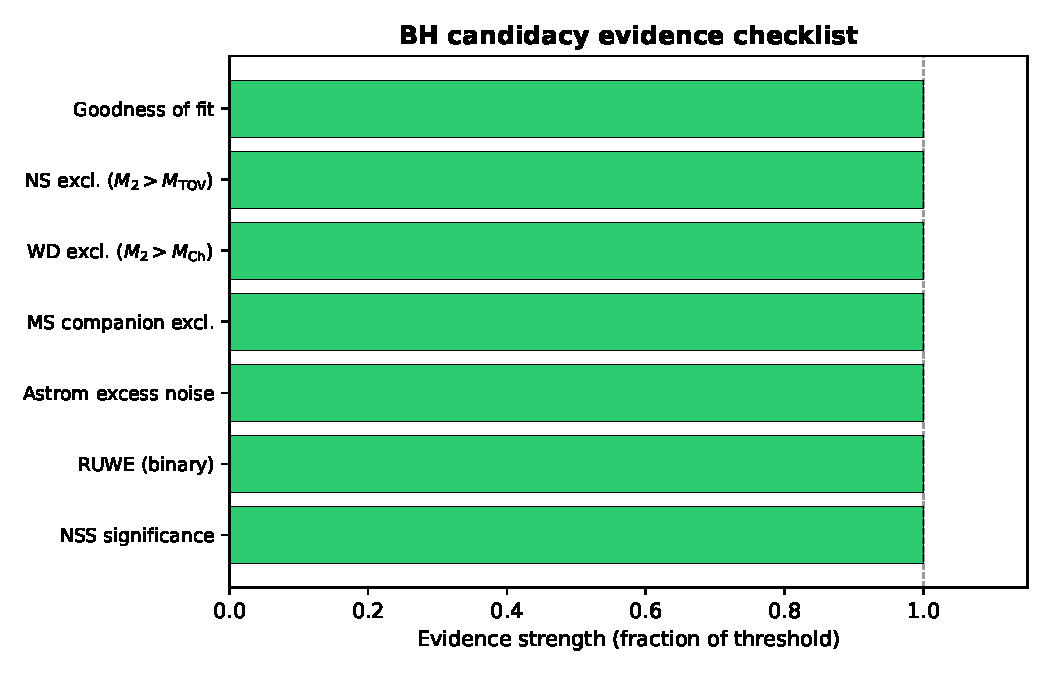
\includegraphics[width=\textwidth]{figures/fig_checklist.pdf}
\caption{Evidence checklist for BH candidacy.}
\label{fig:checklist}
\end{figure*}

% ====================================================================
\label{lastpage}
\end{document}
